\documentclass[12pt,addpoints,answers]{exam}
\usepackage[utf8]{inputenc}

\unframedsolutions
\renewcommand{\solutiontitle}{\noindent\textbf{Solution:}\par\noindent}
\SolutionEmphasis{\color{blue}}
%\noprintanswers

\usepackage{booktabs}
\usepackage{tabularx}
\usepackage{url}
\usepackage{xfrac}

\usepackage{siunitx}
\sisetup{parse-numbers=false}

\usepackage{listings}
\lstset{basicstyle=\ttfamily}

\usepackage{tikz}
\usetikzlibrary{arrows}
\usetikzlibrary{decorations.pathreplacing}
\usetikzlibrary{chains}
\usetikzlibrary{positioning}
%\tikzset{>=stealth',every on chain/.append style={join}, every join/.style={-,blue,thick,dashed}}

\usepackage{float}

% Used for code embed in problem 3
\usepackage{listings}
\usepackage{color}
\usepackage{amsmath}

\title{Computer Networks Homework 5}
\author{Spring 2020}
\date{Due: 20 April 2020}

\begin{document}
\maketitle

\begin{questions}
\question[8] In ASCII, the base set of characters are encoded as 7-bit values (with the most significant bit being 0). You can confirm this for yourself by referencing a resource such as \url{asciitable.com}. We can take advantage of this fact when calculating two-dimensional parity. Instead of adding a new bit to represent each row's parity, we instead "borrow" this most significant bit for the partiy calculation.

Calculate the two-dimensional parity for the ASCII string \lstinline[showspaces=true]{MTU 1885}, noting that the string has 8 characters including the space. Encode the row parity for each 7-bit ASCII character in the most significant bit of the string. List the encoded message as a string of bytes in hexidecimal.
\begin{solution}
	Calculating parities:
	\begin{table}[H]
		\centering
		\caption{}
		\label{tab:my-table}
		\begin{tabular}{|c|cccccccc|c|}
			\hline
			Letter &
			\multicolumn{1}{c|}{0th} &
			\multicolumn{1}{c|}{1st} &
			\multicolumn{1}{c|}{2nd} &
			\multicolumn{1}{c|}{3rd} &
			\multicolumn{1}{c|}{4th} &
			\multicolumn{1}{c|}{5th} &
			\multicolumn{1}{c|}{6th} &
			7th &
			Parity \\ \hline
			M   & 0 & 1 & 0 & 0 & 1 & 1 & 0 & 1 & 0 \\ \cline{1-1} \cline{10-10} 
			T   & 0 & 1 & 0 & 1 & 0 & 1 & 0 & 0 & 1 \\ \cline{1-1} \cline{10-10} 
			U   & 0 & 1 & 0 & 1 & 0 & 1 & 0 & 1 & 1 \\ \cline{1-1} \cline{10-10} 
			' ' & 0 & 0 & 1 & 0 & 0 & 0 & 0 & 0 & 1 \\ \cline{1-1} \cline{10-10} 
			1   & 0 & 0 & 1 & 1 & 0 & 0 & 0 & 1 & 1 \\ \cline{1-1} \cline{10-10} 
			8   & 0 & 0 & 1 & 1 & 1 & 0 & 0 & 0 & 1 \\ \cline{1-1} \cline{10-10} 
			8   & 0 & 0 & 1 & 1 & 1 & 0 & 0 & 0 & 1 \\ \cline{1-1} \cline{10-10} 
			5   & 0 & 0 & 1 & 1 & 0 & 1 & 0 & 1 & 0 \\ \hline
			Parity &
			\multicolumn{1}{c|}{0} &
			\multicolumn{1}{c|}{1} &
			\multicolumn{1}{c|}{1} &
			\multicolumn{1}{c|}{0} &
			\multicolumn{1}{c|}{1} &
			\multicolumn{1}{c|}{0} &
			\multicolumn{1}{c|}{0} &
			0 &
			\\ \hline
		\end{tabular}
	\end{table}
New bit strings
\begin{table}[H]
	\centering
	\caption{}
	\label{tab:my-table}
	\begin{tabular}{|c|cccccccc|c|}
		\hline
		Letter &
		\multicolumn{1}{c|}{0th} &
		\multicolumn{1}{c|}{1st} &
		\multicolumn{1}{c|}{2nd} &
		\multicolumn{1}{c|}{3rd} &
		\multicolumn{1}{c|}{4th} &
		\multicolumn{1}{c|}{5th} &
		\multicolumn{1}{c|}{6th} &
		7th &
		Hex \\ \hline
		M   & 0 & 1 & 0 & 0 & 1 & 1 & 0 & 1 & 4D \\ \cline{1-1} \cline{10-10} 
		T   & 1 & 1 & 0 & 1 & 0 & 1 & 0 & 0 & D4 \\ \cline{1-1} \cline{10-10} 
		U   & 1 & 1 & 0 & 1 & 0 & 1 & 0 & 1 & D5 \\ \cline{1-1} \cline{10-10} 
		' ' & 1 & 0 & 1 & 0 & 0 & 0 & 0 & 0 & A0 \\ \cline{1-1} \cline{10-10} 
		1   & 1 & 0 & 1 & 1 & 0 & 0 & 0 & 1 & B1 \\ \cline{1-1} \cline{10-10} 
		8   & 1 & 0 & 1 & 1 & 1 & 0 & 0 & 0 & B8 \\ \cline{1-1} \cline{10-10} 
		8   & 1 & 0 & 1 & 1 & 1 & 0 & 0 & 0 & B8 \\ \cline{1-1} \cline{10-10} 
		5   & 0 & 0 & 1 & 1 & 0 & 1 & 0 & 1 & 35 \\ \cline{1-1} \cline{10-10} 
	\end{tabular}
\end{table}

Final String: \textbf{4DD4D5A0B1B8B835}
\end{solution}

\question Perform the following operations using carry-free binary. \emph{Please show your work.}
\begin{parts}
\part[3] $100111_2 + 011101_2$
\begin{solution}
\begin{table}[H]
	\centering
	\caption{}
	\label{tab:my-table}
	\begin{tabular}{|l|llllllll}
		\hline
		Bit &
		\multicolumn{1}{l|}{0} &
		\multicolumn{1}{l|}{1} &
		\multicolumn{1}{l|}{2} &
		\multicolumn{1}{l|}{3} &
		\multicolumn{1}{l|}{4} &
		\multicolumn{1}{l|}{5} &
		\multicolumn{1}{l|}{6} &
		\multicolumn{1}{l|}{7} \\ \hline
		Byte 1   & 0 & 0 & 1 & 0 & 0 & 1 & 1 & 1 \\ \cline{1-1}
		Byte 2   & 0 & 0 & 0 & 1 & 1 & 1 & 0 & 1 \\ \cline{1-1}
		Addition & 0 & 0 & 1 & 1 & 1 & 2 & 1 & 2 \\ \cline{1-1} \hline
		Result   & 0 & 0 & 1 & 1 & 1 & 0 & 1 & 0 \\ \cline{1-1}
	\end{tabular}
\end{table}
\end{solution}

\part[3] $011110_2 - 111110_2$
\begin{solution}
\end{solution}

\part[3] $10010_2 \times 10101_2$
\begin{solution}
	\begin{table}[H]
		\centering
		\caption{}
		\label{tab:my-table}
		\begin{tabular}{|l|llllllll}
			\hline
			Bit &
			\multicolumn{1}{l|}{0} &
			\multicolumn{1}{l|}{1} &
			\multicolumn{1}{l|}{2} &
			\multicolumn{1}{l|}{3} &
			\multicolumn{1}{l|}{4} &
			\multicolumn{1}{l|}{5} &
			\multicolumn{1}{l|}{6} &
			\multicolumn{1}{l|}{7} \\ \hline
			Byte 1   & 0 & 0 & 1 & 0 & 0 & 1 & 1 & 1 \\ \cline{1-1}
			Byte 2   & 0 & 0 & 0 & 1 & 1 & 1 & 0 & 1 \\ \cline{1-1}
			Addition & 0 & 0 & 1 & 1 & 1 & 2 & 1 & 2 \\ \cline{1-1} \hline
			Result   & 0 & 0 & 1 & 1 & 1 & 0 & 1 & 0 \\ \cline{1-1}
		\end{tabular}
	\end{table}
\end{solution}
\part[3] $1111111_2 + 1111111_2$
\begin{solution}
	\begin{table}[H]
		\centering
		\caption{}
		\label{tab:my-table}
		\begin{tabular}{|l|llllllll}
			\hline
			Bit &
			\multicolumn{1}{l|}{0} &
			\multicolumn{1}{l|}{1} &
			\multicolumn{1}{l|}{2} &
			\multicolumn{1}{l|}{3} &
			\multicolumn{1}{l|}{4} &
			\multicolumn{1}{l|}{5} &
			\multicolumn{1}{l|}{6} &
			\multicolumn{1}{l|}{7} \\ \hline
			Byte 1   & 0 & 1 & 1 & 1 & 1 & 1 & 1 & 1 \\ \cline{1-1}
			Byte 2   & 0 & 1 & 1 & 1 & 1 & 1 & 1 & 1 \\ \cline{1-1}
			Addition & 0 & 2 & 2 & 2 & 2 & 2 & 2 & 2 \\ \cline{1-1} \hline
			Result   & 0 & 1 & 1 & 1 & 1 & 1 & 1 & 1 \\ \cline{1-1}
		\end{tabular}
	\end{table}
\end{solution}
\end{parts}

\question[8] Calculate the CRC checksum for the data $100111110011_2$ and the CRC-8 polynomial $x^8 + x^2 + x + 1$.
\begin{solution}
	Polynomial Bitstring
\begin{table}[H]
	\centering
	\caption{}
	\label{tab:my-table}
	\begin{tabular}{|c|ccccccccc}
		\hline
		Bits &
		\multicolumn{1}{c|}{0} &
		\multicolumn{1}{c|}{1} &
		\multicolumn{1}{c|}{2} &
		\multicolumn{1}{c|}{3} &
		\multicolumn{1}{c|}{4} &
		\multicolumn{1}{c|}{5} &
		\multicolumn{1}{c|}{6} &
		\multicolumn{1}{c|}{7} &
		\multicolumn{1}{c|}{8} \\ \hline
		Polynomial &
		x\textasciicircum{}8 &
		&
		&
		&
		&
		&
		x\textasciicircum{}2 &
		x &
		1 \\ \cline{1-1}
		BitString &
		1 &
		0 &
		0 &
		0 &
		0 &
		0 &
		1 &
		1 &
		1 \\ \cline{1-1}
	\end{tabular}
\end{table}
	\definecolor{dkgreen}{rgb}{0,0.6,0}
\definecolor{gray}{rgb}{0.5,0.5,0.5}
\definecolor{mauve}{rgb}{0.58,0,0.82}
\lstset{frame=tb,
	language=Python,
	aboveskip=3mm,
	belowskip=3mm,
	showstringspaces=false,
	columns=flexible,
	basicstyle={\small\ttfamily},
	numbers=none,
	numberstyle=\tiny\color{gray},
	keywordstyle=\color{blue},
	commentstyle=\color{dkgreen},
	stringstyle=\color{mauve},
	breaklines=true,
	breakatwhitespace=true,
	tabsize=4
}
\begin{lstlisting}
def crc_remainder(input_bitstring, polynomial_bitstring, initial_filler):
	'''
	Calculates the CRC remainder of a string of bits using a chosen polynomial.
	initial_filler should be '1' or '0'.
	'''
	polynomial_bitstring = polynomial_bitstring.lstrip('0')
	len_input = len(input_bitstring)
	initial_padding = initial_filler * (len(polynomial_bitstring) - 1)
	input_padded_array = list(input_bitstring + initial_padding)
	while '1' in input_padded_array[:len_input]:
		cur_shift = input_padded_array.index('1')
		for i in range(len(polynomial_bitstring)):
			input_padded_array[cur_shift + i] = str(int(polynomial_bitstring[i] != input_padded_array[cur_shift + i]))
	return ''.join(input_padded_array)[len_input:]
crc_remainder('100111110011', '100000111', '0')
\end{lstlisting}

Result: \textbf{01101010}
\end{solution}

\question Consider the following extended LAN consisting of three hosts (X, Y, and Z) and three learning bridges (B1, B2, B3). Assume that the bridges initially have empty forwarding tables, will fill their forwarding table with the source address from any incoming packet, and will broadcast any packet for which is missing a forwarding entry. Answer the following questions about the hosts and bridges cumulatively, e.g., part (b) occurs after part (a).
\begin{center}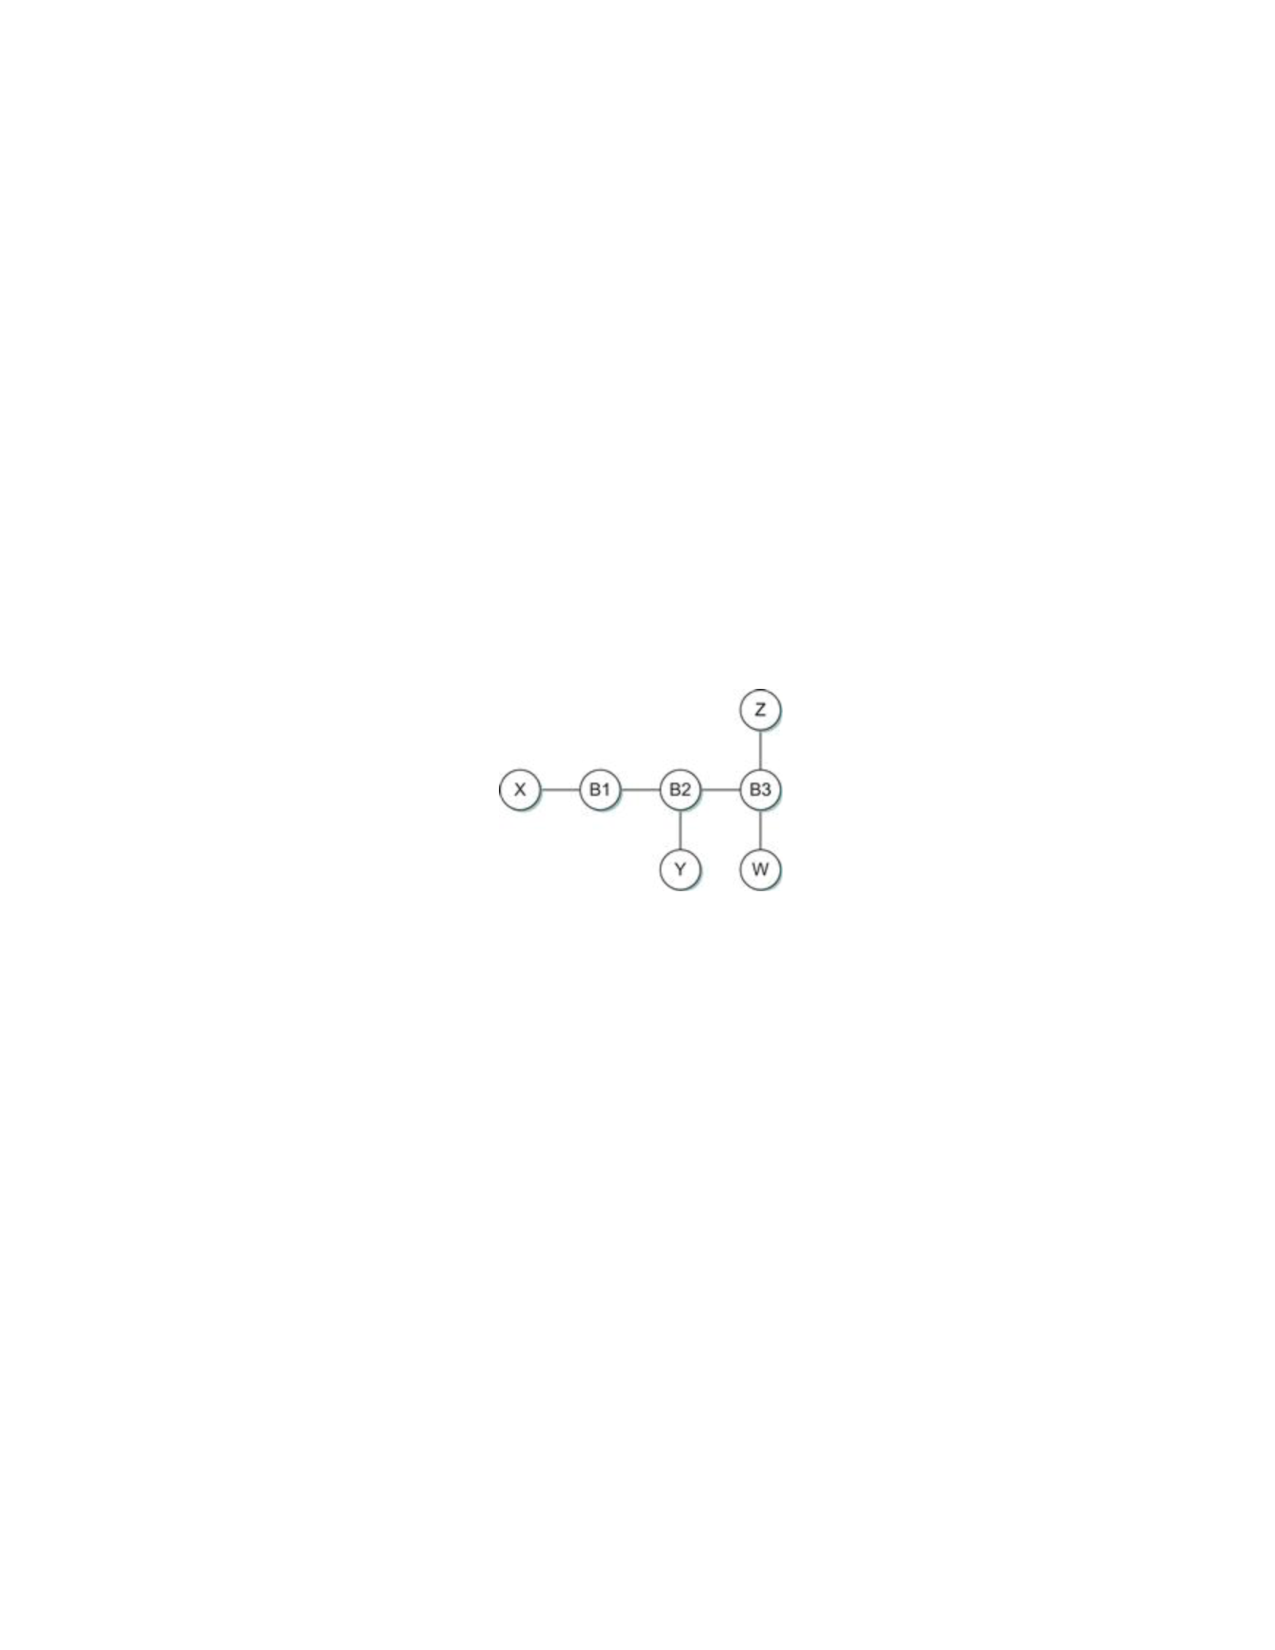
\includegraphics[width=0.35\linewidth]{fig/simple.pdf}\end{center}
\begin{parts}
\part[3] Suppose X sends a packet destined for W. Which bridges learn where X is? Does Y's network interface see this packet?
\begin{solution}
	Bridge 2 learns where Host W is from Bridge 3.  So cumulatively bridges 1, 2, and 3.
	
	Host Y does not see this packet as it doesn't check in to Bridge 2 unless it's sending and expecting something back. Presumably at this point, no bridge is aware yet of Host Y.
\end{solution}

\part[3] Suppose Z sends a packet destined for X. Which bridges learn where Z is? Does Y's network interface see this packet? Presumably at this point, no bridge is aware yet of Host Y.
\begin{solution}
	Bridge 2 learns where Host X is from Bridge 1. So cumulatively bridges 1, 2, and 3.
	
	Host Y does not see this packet as it doesn't check in to Bridge 2 unless it's sending and expecting something back.
\end{solution}

\part[3] Suppose Y sends a packet destined for X. Which bridges learn where Y is? Does Z's network interface see this packet?
\begin{solution}
	Bridge 2 and Bridge 1 find where Y is.
	
	Host Z does not see this packet as it doesn't check in to Bridge 2 unless it's sending and expecting something back.
\end{solution}

\part[3] Suppose W sends a packet destined for Y. Which bridges learn where W is? Does Z's network interface see this packet?
\begin{solution}
	Bridge 1,2, and 3 learn where W is.
	
	Host Z does not see this packet as it doesn't check in to Bridge 2 unless it's sending and expecting something back.
\end{solution}
\end{parts}

\question The following extended LAN has just come back online after a power outage and the bridges now need to agree on a spanning tree for propagating Ethernet frames
\begin{center}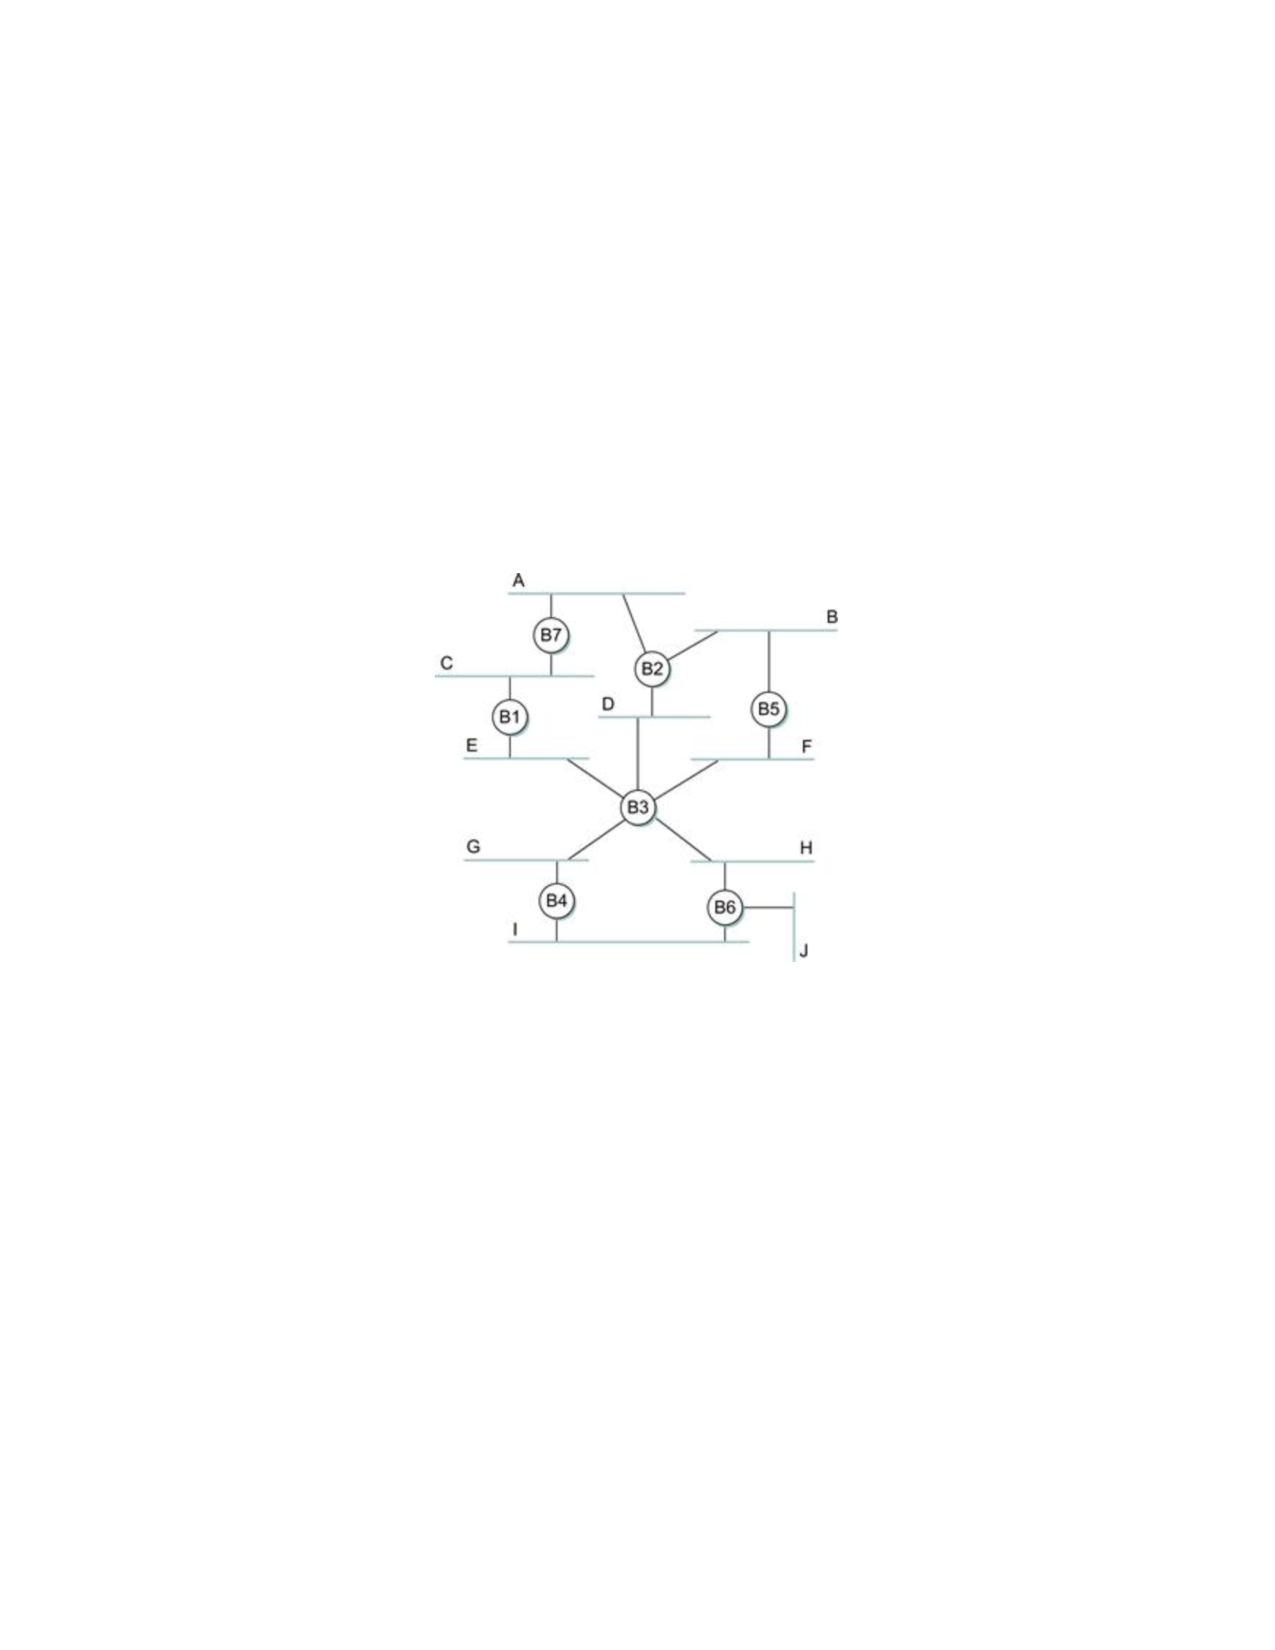
\includegraphics[width=0.45\linewidth]{fig/complex.pdf}\end{center}
\begin{parts}
\part[3] Indicate the category of each port (root, designated, blocked) for every bridge. As a human, you do not need to run the distributed spanning tree protocol exactly---just provide the end result based on the rules and preferences of the algorithm.
\begin{solution}
		\begin{enumerate}
		\item Bridge 1
		\begin{enumerate}
			\item Port C: Designated
			\item Port E: Root
		\end{enumerate}
	\end{enumerate}
	
	\begin{enumerate}
		\item Bridge 2
		\begin{enumerate}
			\item Port A: Designated
			\item Port B: Designated
			\item Port D: Root
		\end{enumerate}
	\end{enumerate}
	
	\begin{enumerate}
		\item Bridge 3
		\begin{enumerate}
			\item Port E: Designated
			\item Port F: Designated
			\item Port G: Designated
			\item Port H: Designated
		\end{enumerate}
	\end{enumerate}
	
	\begin{enumerate}
		\item Bridge 4
		\begin{enumerate}
			\item Port G: Root
			\item Port I: Blocked
		\end{enumerate}
	\end{enumerate}
	
	\begin{enumerate}
		\item Bridge 5
		\begin{enumerate}
			\item Port B: Blocked
			\item Port F: Root
		\end{enumerate}
	\end{enumerate}
	
	\begin{enumerate}
		\item Bridge 6
		\begin{enumerate}
			\item Port H: Root
			\item Port I: Designated
			\item Port J: Designated
		\end{enumerate}
	\end{enumerate}
	
	\begin{enumerate}
		\item Bridge 7
		\begin{enumerate}
			\item Port A: Blocked
			\item Port C: Root
		\end{enumerate}
	\end{enumerate}
\end{solution}

\part[7] Some time after establishing the spanning tree from part (a), bridge B2 suffers a catastrophic failure. Indicate the category of each port (root, designated, blocked) after the recovery process and a new spanning tree has been formed.
\begin{solution}
	\begin{enumerate}
	\item Bridge 1
	\begin{enumerate}
		\item Port C: Designated
		\item Port E: Root
	\end{enumerate}
\end{enumerate}

\begin{enumerate}
	\item Bridge 2
	\begin{enumerate}
		\item Port A: Blocked
		\item Port B: Blocked
		\item Port D: Root
	\end{enumerate}
\end{enumerate}

\begin{enumerate}
	\item Bridge 3
	\begin{enumerate}
		\item Port E: Designated
		\item Port F: Designated
		\item Port G: Designated
		\item Port H: Designated
	\end{enumerate}
\end{enumerate}

\begin{enumerate}
	\item Bridge 4
	\begin{enumerate}
		\item Port G: Root
		\item Port I: Blocked
	\end{enumerate}
\end{enumerate}

\begin{enumerate}
	\item Bridge 5
	\begin{enumerate}
		\item Port B: Designated
		\item Port F: Root
	\end{enumerate}
\end{enumerate}

\begin{enumerate}
	\item Bridge 6
	\begin{enumerate}
		\item Port H: Root
		\item Port I: Designated
		\item Port J: Designated
	\end{enumerate}
\end{enumerate}

\begin{enumerate}
	\item Bridge 7
	\begin{enumerate}
		\item Port A: Designated
		\item Port C: Root
	\end{enumerate}
\end{enumerate}
\end{solution}
\end{parts}


\end{questions}
\end{document}
